\documentclass[11pt]{article}
\usepackage{palatino}
\usepackage{graphicx}
%\usepackage{wrapfig}
\usepackage[top=1in, bottom=1in, left=0.5in, right=0.5in]{geometry}
\newcommand{\BibTeX}{{\sc Bib}\TeX}
\begin{document}
\title{Rube Goldber Simulation: Trap of the tomb of the Pharoah Tutankhamun : A CS296 Group 19 Report}
\author{Tarun Kathuria \\ 110110028 \\ \texttt{tarunkathuria@gmail.com} \and Rohith Kishan \\ 110050071 \\ \texttt{krsrk@cse.iitb.ac.in} \and Vikash Challa \\ 110050077 \\ \texttt{vikash@cse.iitb.ac.in}}
\date{\today}
\maketitle

\section{Introduction}

We now present our Rube Goldberg Simulation\cite{wikirgm} "Trap of the tomb of the Pharaoh Tutankhamun". 
This physics simulation has been developed using C++, a physics engine called Box2D developed by Mr. Erin Catto and elements of OpenGL(GLUT) for rendering the graphics. This simulation has been created as part of our \underline{CS296 project}. When such a Box2D simulation is observed, it is often breathtaking to view and we hope that you have as much fun watching it as we had while making it.

\section{Original Design}

When we initially learnt about Box2D and our project at the beginning of the semester, we looked into quite a few online Rube Goldberg Machines(primarily from YouTube\cite{rubegoldbergYouTube}). Our original design that was created at the beginning of the semester included quite a few parts. The main moving objects are described below:

\subsection{The starting ball and the Newton's Cradle}

\begin{itemize}
	\item Firstly, the person standing below pulls a string accidently and causes the pulley system to move. 
	\item The string on the pulley is connected to a small ball which moves to the left under the force of the pull. 
	\item It stops once it reaches a rod which is hinged. This rod now rotates down to hit a Newton's cradle system and which hit a blue boulder at rest at the right side. 
	\item This blue boulder then starts moving to the right and then falls down.
\end{itemize}

\subsection{Pulley system and the falling balls}

\begin{itemize}
	\item The blue boulder from the previous subsubsection falls into a bucket which is attached at one end of a 2-pulley system.
	\item On the other side, there is another bucket which is tilted downwards and has a few heavy balls but do not fall down since there is a huge vertical strip blocking the balls from falling. 
	\item This strip is connected to the string of the 2-pulley system. When the blue boulder falls into the bucket, that bucket starts moving down and, therefore, this strip starts moving up allowing the balls to fall freely.
	\item Along with this, there is a bucket suspended in mid-air using age-old, forgotten Egyptian technology. When the balls fall into this bucket, the bucket starts falling down.
	\end{itemize}
\subsection{See-saw and the ball and the dominoes, marbles and the revolving platforms}

\begin{itemize}
\item We get to see another prime example of age-old, forgotten Egyptian technology here.
\item The bucket of the balls falls on the right side of the plank of the see-saw. 
 \item On the left side, there is small ball with weightlessness capabilites. 
 \item It is attached to the plank using a special sort of glue and while the see-saw rotates after the bucket falls on the right side of the plank, this ball slowly moves to the edge of the plank(it's glue evaporating due to friction and other moist environments often found in pyramids). 
 \item This ball finally loses contact from the plank and with some impulse, starts moving to the right.

\item The weightless ball then goes and hits a domino from a cluster of a few which causes all the dominoes to topple. 
\item The weightless ball then continues to float upwards as weightless objects do. When the final domino falls it hits a tilted appendage blocking the a few small marbles.
\item This appendage then moves creating a path for the marbles to roll onto a platform. Two of these marbles fall into a ditch slightly ahead. A third falls into another ditch slightly ahead of the previous ditch.
\item The final marble then rolls over this marble(in the ditch) and falls off the right onto a few revolving platforms.
\item When the marble falls on the first revolving platform, that platform starts revolving around it's center which causes this marble to fall onto another platform below it and so on until finally it falls off the final platform.
\end{itemize}

\subsection{Conveyor Belt, Huge Boulders, Hinged structure and the person's eventual doom}
\begin{itemize}
	\item Finally, the marble falls onto a conveyor belt with a support to store things. 
	\item The marble then starts moving with the conveyor belt and is thrown to the left when the support starts moving down again. This marble then hits a huge boulder with an extremely high impulse and the boulder slowly starts moving down to roll over the person who triggered the trap. 
	\item Seeing the boulder, the person may try to run to the left and that is where our weightless bucket of balls from the previous subsubsection comes into play.
	\item That bucket fell into another container which was very intricately hinged to block a boulder from falling down.
	\item Due to this bucket falling and due to rusty joints, the hinged structure slowly makes way for the boulder to fall through and if the person tried to run to the left, he would be crushed by this boulder then!
	\item However, to give the human a fighting chance, he has the ability to move left or right using the 'a' and 'd' keys.
\end{itemize}


\section{Final Design}
Initial designs are often made optimistically and in our case involved elements which didn't exactly match the laws of physics. Therefore, we decided to drop those ideas in the final simulation that we have created. Everything remains the same except:
\subsection{Intricately hinged container}
\begin{itemize}
\item The intricately hinged container blocking the other boulder from killing the person just cannot exist in real life because such objects due to being hinged, will obviously give way under the sheer force of the big boulder holding it and therefore, will rollover before the other boulder has a chance to kill the guy. 
\item That being said, we can't allow the guy to live now can we? So we have made a huge chasm a few kilometres to the left of the person. If the boulder doesn't kill him, due to poor lighting in Egyptian tombs, he falls into the chasm and continues on for a few hundred kilometres and meets his doom! 
\end{itemize}
\subsection{Marbles}
	\begin{itemize}
	\item The dominoes toppling and causing an appendage to fall down, creating a path for the marbles to flow down is not physically possible since the appendage would fall in the other direction and the marbles wouldn't land on the platform. 
	\item That is why, we have made the dominoes directly hit one marble which hits the other and so on... 
	\item The rest of the simulation remains roughly the same.
	\end{itemize}
\section{Final comments on our design}
Our design was primarily based on our fascination with Egyptian mummies, tombs and pyramids. It is popular belief that tombs of pharoahs were built in pyramids with intricate traps to stop any grave-robbers. Egyptians being as awesome as they are like to build breathtaking things(see the pyramids themselves), wanted to design intricate yet breathtaking traps for the same and it feels that designing something like a Rube Goldberg Machine for the same might be a good idea.
\subsection{Interesting features about our design}
\begin{itemize}
	\item Conveyor belt : A conveyor belt is very useful in many things and acts as a great source of the high impulse that was needed to knock off that big boulder from it's pedestal using a marble much smaller and lighter than that.
	\item Newton's cradle : A very famous example of a device demonstrating the law of conservation of momentum and energy, it acts as a nice way to transfer energy from one place to another.
	\item The intricately hinged structure : While it does not follow the laws of physics properly, it is in our opinion, quite a nice way to create a double trap to kill the person. Perhaps a slight modification to the same, might yield a physically possible solution later on...
\end{itemize}

\section{Timing Inferences}
After creating the simulation, it is also necessary to profile the code and see if any improvements are possible. In this section, we generate plots and see how the time-related metrics change.
Finally, we perform profiling inferences on the executables to detect bottlenecks in the code and draw inferences based on them. We finally conclude with some suggestions on how to optimize the code. \\
There are 4 time-related metrics we are primarily concerned with:

 Loop Time
 
 Step Time
 
 Velocity Updates Time
 
 Position Updates Time


We first analyse the time-related metrics when there is very little CPU load on the computer.

\begin{figure}[h!]
\caption{Loop Time,Step Time v/s Iteration values}
\centering
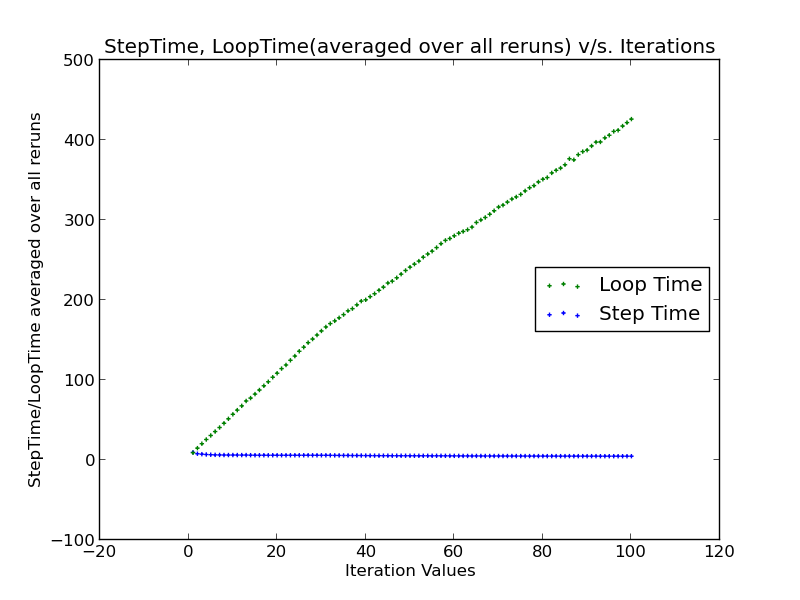
\includegraphics[height=8cm]{images/g19_proj_plot01}
\end{figure}

\subsection{Loop Time}



\begin{itemize}
	\item When averaged over all reruns, Loop Time increases linearly upto the 30th iteration. Beyond that a slight decrease of slope is observed but the graph still stays linear only. 
	\item This is not surprising since initially the simulation starts out slower. However, as the number of iterations increases, the rate at which the simulation happens increases and therefore, the loop time grows slower with increase in iterations.
	\item When averaged over all iterations, Loop Time remains almost constant with respect to the rerun numbers but some jumps do creep in.
	\item This is clearly not a surprise since the metrics should not vary with reruns.	
\end{itemize}

\begin{figure}[h!]
\caption{Loop Time,Step Time v/s Rerun values}
\centering
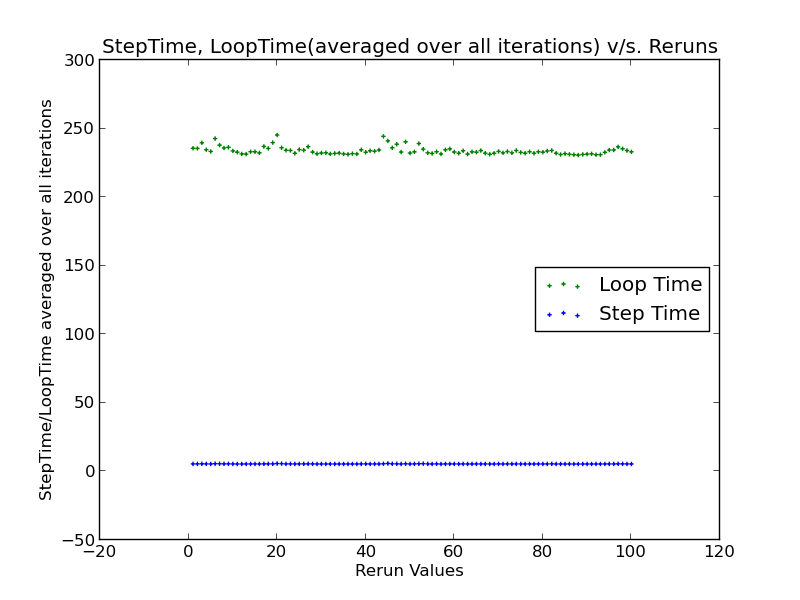
\includegraphics[height=8cm]{images/g19_proj_plot03}
\end{figure}
\begin{figure}[h!]
\caption{Step Time v/s Iteration values with Error bars}
\centering
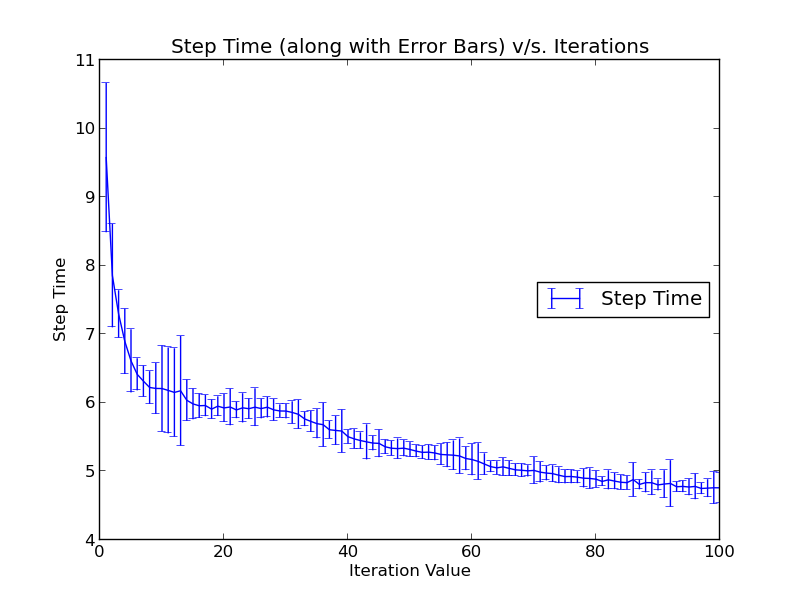
\includegraphics[height=8cm]{images/g19_proj_plot05}
\end{figure}
\subsection{Step Time}
	\begin{itemize}
		\item Step Time also,when averaged over all reruns, decreases sharply till iteration number 30 and beyond that decreases slowly.
		\item Initially, the simulation is slower and therefore, the step time is larger. However, as iteration values increase, the simulation becomes faster and therefore, the step time decreases at a faster rate.
		\item The step time(averaged over all iterations) decreases at a very slow rate as the rerun number changes, unsurprisingly.
	\end{itemize}


	
\subsection{Velocity Updates Time}
	\begin{itemize}
		\item The velocity updates time(averaged over all reruns) stays almost the same till iteration number 30 and then decreases at a rate which is roughly polynomial.
		\item This is easily explained since the simulation starts out slower and ,thus, the time taken for velocity updates are larger. Beyond iteration number 30, the simulation increases at a fast rate and ,therefore, the velocity updates time goes down
		\item Unsurprisingly, the velocity updates time(averaged over all iterations) does not vary considerably as the rerun number changes.
		\item The velocity updates time(averaged over all iterations) does not vary considerably as the rerun number changes because the simulation is being carried out with the same iteration value, only the rerun happens again and since the CPU load is almost constant, a different rerun does not cause this value to vary considerably.
	\end{itemize}
\begin{figure}[h!]
\caption{Velocity, Position Update,Collision and Step Times v/s iteration values}
\centering
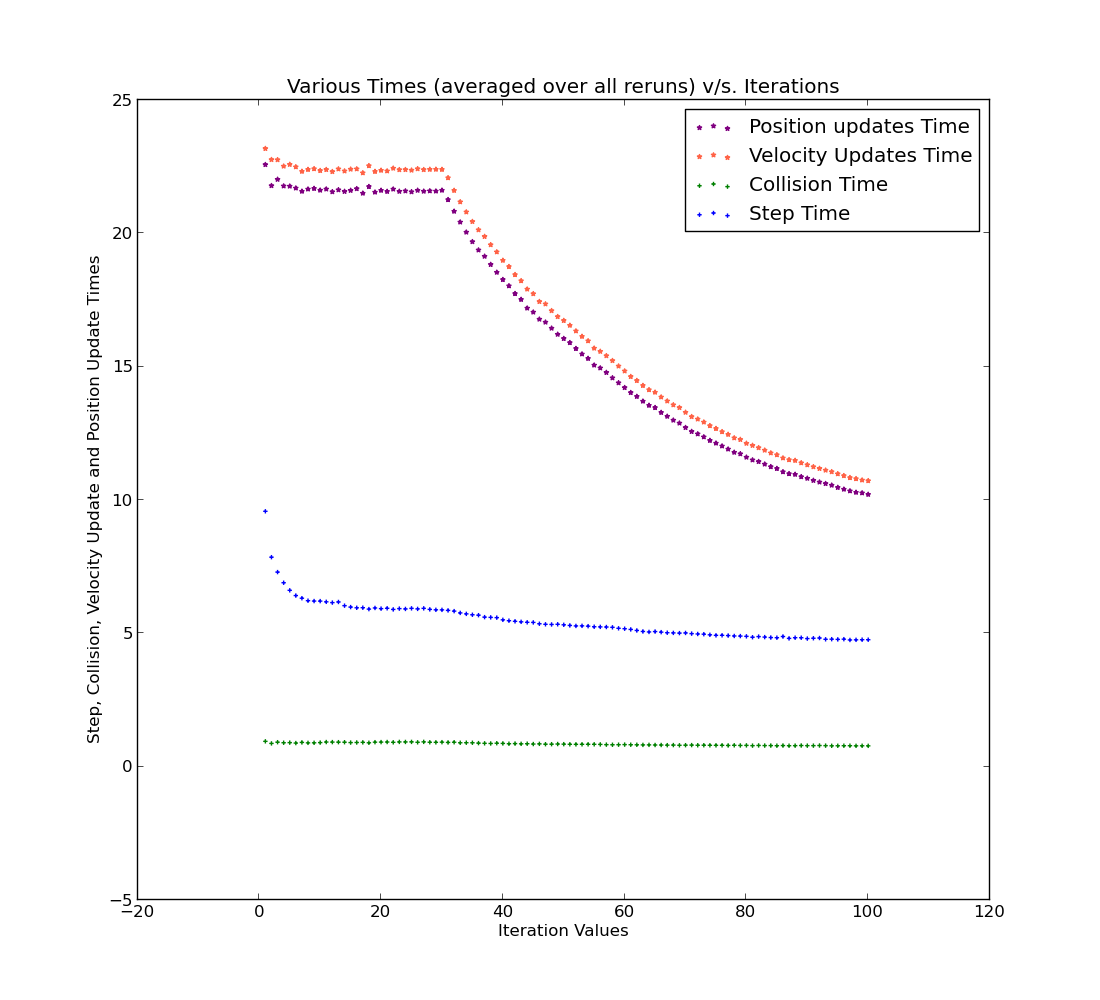
\includegraphics[height=8cm]{images/g19_proj_plot02}
\end{figure}
\subsection{Position Updates Time}
	\begin{itemize}
		\item The position updates time(averaged over all reruns) stays almost the same till iteration number 30 and then decreases at a rate which is roughly polynomial.
		\item This is easily explained since the simulation starts out slower and ,thus, the time taken for position updates are larger. Beyond iteration number 30, the simulation increases at a fast rate and ,therefore, the position updates time goes down
		\item Unsurprisingly, the position updates time(averaged over all iterations) does not vary considerably as the rerun number changes.
		\item The position updates time(averaged over all iterations) does not vary considerably as the rerun number changes because the simulation is being carried out with the same iteration value, only the rerun happens again and since the CPU load is almost constant, a different rerun does not cause this value to vary considerably.
	\end{itemize}
\begin{figure}[h!]
\caption{Velocity, Position Update,Collision and Step Times v/s rerun values}
\centering
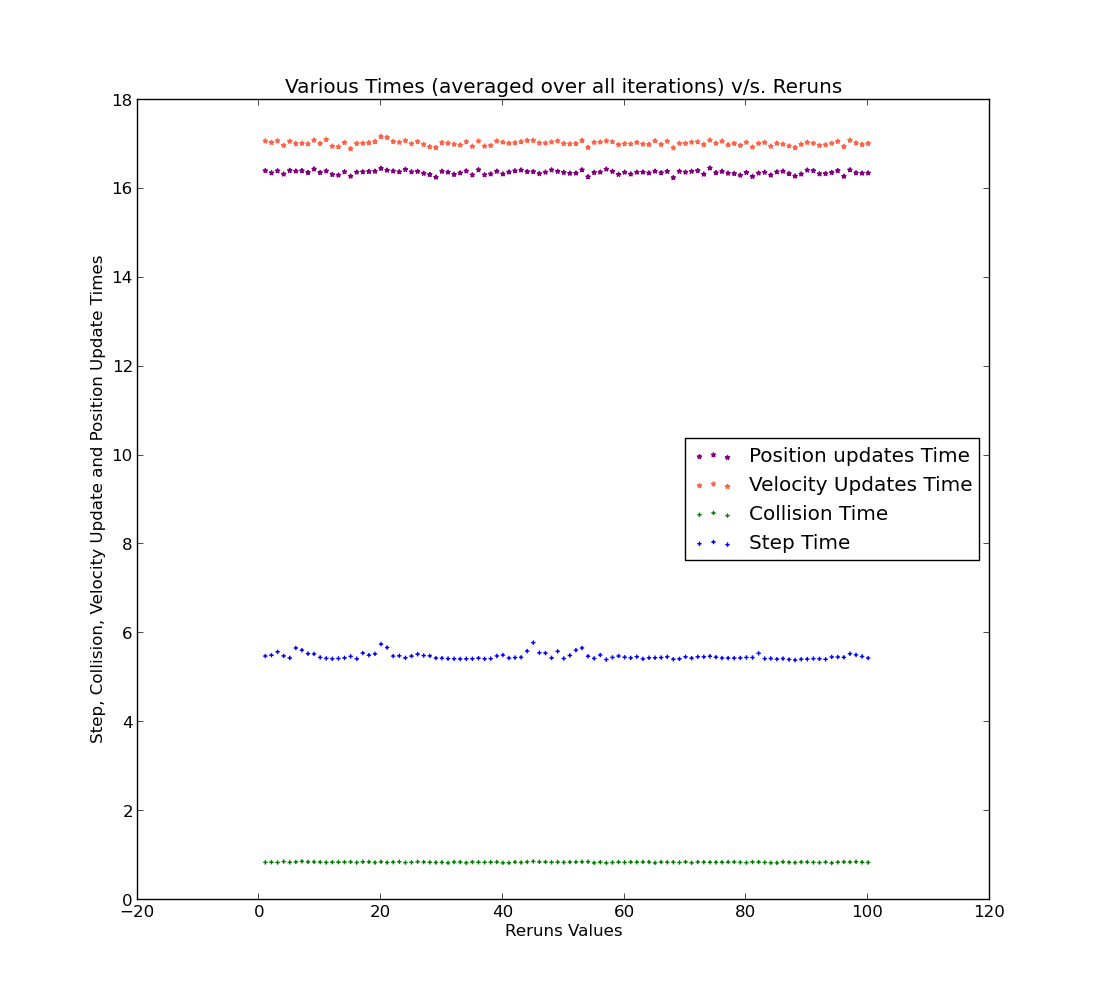
\includegraphics[height=8cm]{images/g19_proj_plot04}
\end{figure}

\section{Profiling Inferences}
We perform profiling experiments using a famous profiling tool called gprof and draw inferences based on the reports and call graphs generated by them. 2 experiments are carried out. In each of them, Box2D is compiled using a different mode:
	
	
	
		 Debug Version
	
	
		 Release Version
	
	
	
	For each of the 2 versions, profiling of the executable is done using gprof and then a gprof report and a call graph is generated which are used to identify the bottlenecks in the code and realise how optimizing the code makes a difference.
	\subsection{Debug Version}
		\begin{itemize}
		\item In the first experiment, Box2D is compiled using the Debug Build Type and no optimization flags are added while compiling the code. 
		\item From the call graph and the gprof report, we realise the main functions which use most of the cycles of the code.
		\item These are shown in the profile report which is provided along with this report.
\item As is evident, the b2ContactSolver::SolveVelocityConstraints, b2World::SolveTOI, various constructors and operators are the main bottlenecks of the debug version. The b2Vec, b2World etc. are part of Box2D and can't really be optimized further. 
\item However, the other things give us useful insight on the code that has been written. Specifically, we observe that the constructors are being called many times and the operators as well.
\item  Perhaps they can be optimized ? This will become more clear after the results of the Release version of the experiment are presented.
\item Shown below is the call graph of the debug version and this is essentially the same data as the profile report shown above but is useful in realising which function calls which other functions.
\end{itemize}
\begin{figure}[h!]
\caption{Call Graph for the Debug version}
\centering
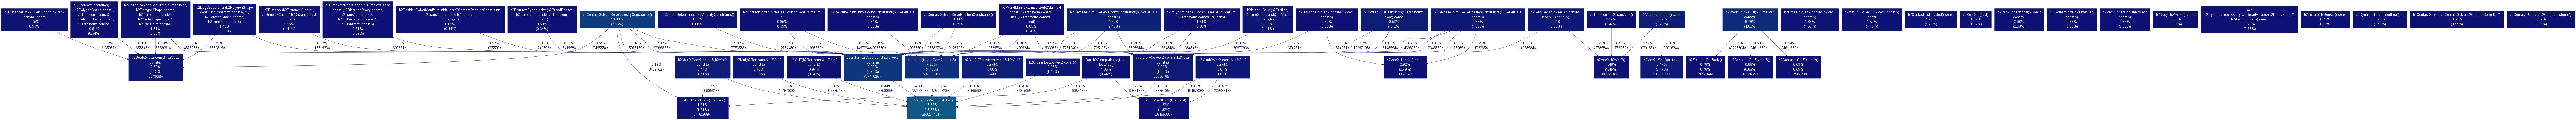
\includegraphics[width=\linewidth,height=2.5cm]{images/callgraphdebug}
\end{figure}
	\subsection{Release Version}
		\begin{itemize}
		\item We now run the experiment with Box2D compiled using the Release Build Type and the optimization flag -O3 is used while compiling the code. 
		\item The -O3 flag offers many optimizations and include the optimizations of -O1 to -O2 as well. 
		
		\item The executables are smaller and faster since many things have been optimized
	
		\item Instruction scheduling is included and the compiler takes longer to compile and require more memory but it provides maximum optimization without increasing size considerably. This is part of the O2 optimization
		\item The O3 flag turns on the more expensive optimizations like function inlining but increases the size slightly.
		
		\item The main bottlenecks after optimization are shown in the profile report.
		\item From this, we realise that the SolveVelocityConstraints still is the major bottleneck along with SolveTOI but many other initial high cycle-consuming functions have been eliminated. 
		\item A more thorough analysis of this is done in the next subsection which compares the 2 versions.
		\item Like in the Debug version, the call graph for the Release version is shown below.
		\end{itemize}
	\begin{figure}[h!]
	\caption{Call Graph for the Release version}
	\centering
	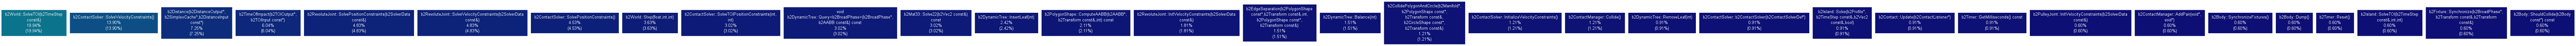
\includegraphics[width=\linewidth,height=0.5cm]{images/callgraphrelease}
	\end{figure}
	\subsubsection{Interpretation of call graphs}
		Call graphs are really just bright, colorful graphs ,albeit, they are extremely useful:
			\begin{itemize}
				\item They show the profile report data in a lot more interesting, visually appealing and helpful manner
				\item They show a parent-child relationship in terms of which function leads to calling of another function
				\item For a parent function, it also along with the time \% consumed by the parent function alone, also shows the total time \% consumed by the parent function and it's children functions.
			\end{itemize}
	\subsection{Comparison of the two versions}
		\begin{itemize}
		\item After observing the profiling reports and call graphs of the two versions, many interesting things are observed. 
		\item Firstly, SolveVelocityConstraints and SolveTOI are major bottlenecks with and without optimization flags. 		\item However, notice that after optimization, the constructors like b2Vec2, b2Cross and b2Dot which were initially amongst the high cycle users do not feature in the high cycle users after optimization. 
		\item Also, after optimization, the +, -, *, / operators which are overloaded in the B2Math.h file are not amongst the high cycle users , whereas they were amongst the top 15 high cycle users in the debug version,i.e., before optimization.
		\item This shows that repeated and unnecessary objects are being created in the native code and unnecessary arithmetic operators are being called when the same thing can be done using lesser calls.
		\item Another thing to observe is that in the Debug version, b2ContactSolver::SolveTOI amounts for 4.85\% of the time cycles, whereas in the Optimized/Release version, this function call constitutes 19.94\% of the time cycles. 
		\item From this we infer that SolveTOI is a major bottleneck and after optimization it is THE major bottleneck in the code. 
		\item This gives us ideas to think about modifying the Box2D source code to try to optimize this function as well as try to reduce the number of calls to this function, if possible since this takes a major amount of time.
		\item Another interesting observation is that the total time taken by the program is a lot lesser in the Release version as compared to the Debug version. 
		\item This is not really surprising since the Release version is the optimized version. The total time taken by the program in the Release version is 3.31 seconds, whereas, in the case of the Debug version, it was 20.43 seconds! 
		\item This shows that the constructors and the overloaded operators were being used in an extremely inefficient manner.
		\end{itemize}
	\subsection{Suggested Optimizations}
		Now we present some of the optimizations that are possible by altering our code as well as that of the Box2D library. A few optimizations are listed below:
		\begin{itemize}
			\item In the main.cpp, to obtain the average time for collisions, velocity updates, position updates, we repeatedly call the pointer to the profile of the virtual world mworld1. This pointer is accessed 4*(number of iterations) times. This can be optimized by storing this pointer in a temporary variable and accessing it from there. This is helpful since pointer accesses are expensive and we are cutting down the time considerably!
			\item Another optimization that can be seen is related to our major bottleneck function, the SolveVelocityConstraints function. In the b2ContactSolver.cpp, on line 402 and 403, 2 b2VelocityContraintPoint pointers cp1 and cp2 are defined. Some attributes of cp1 and cp2 namely, the rB, rA, velocityBias is called many times.
			\item This again leads to many pointer accesses which increase time. A possible solution is to store this attribute in say cp1rA, cp1rB, cp2rA and cp2rB so that they can be directly accessed whenever needed. 
			\item This should bring down the time taken by the SolveVelocityContraints function significantly.
	\end{itemize}


\section{Conclusions}
We had great fun designing the Rube Goldberg Simulation and were satisfied with the results. 
However, there is always scope for improvement and we are sure we will try to make this even better in the future. We hope the reader had as much fun(if not more :) )viewing the simulation as we had while making it. It should be noted that our simulation has been completed primarily due to Prof. Parag Chaudhari, Mr. Erin Catto's user manual\cite{box2dman}
and iforce2d's amazing tutorials\cite{iforce}
\bibliographystyle{plain}
\bibliography{refs}
\end{document}
